%%=============================================================================
%% Resultaten
%%=============================================================================

\chapter{\IfLanguageName{dutch}{Resultaten}{Results}}
\label{ch:resultaten}

\section{Resultaten van de verzamelde data}
Via het formulier van ``JotForm'' waren er 13 inzendingen. Dat lijkt niet veel, maar belangrijk om te weten is dat het invullen ervan behoorlijk lang duurt. Er werd telkens gevraagd om een eigenschap van \textit{elderspeak} na te bootsen door een geluidsfragment in te spreken. Dit is veel werk, waardoor mensen sneller afhaakten.

Toch gaven deze 13 personen 54 audiobestanden ter beschikking. Op die geluidsbestanden kon er gecontroleerd worden of er \textit{elderspeak} aanwezig was.

De data is gelabeld door een persoon, dus het kan zijn dat er fouten in de classificatie van de data slopen zijn. Dit eindwerk is natuurlijk van de richting toegepaste informatica, en niet van een communicatierichting. Een interessante en interdisciplinaire opdracht kan zijn, waarbij studenten verpleegkunde of communicatie nieuwe data labelen en studenten toegepaste informatica testen uitvoeren op de server.

Meer hierover wordt beschreven in wat volgt, namelijk in Hoofdstuk~\ref{ch:vervolg}.

\section{Resultaten na het testen}
De testen worden weergegeven in een \textit{confusion matrix}. Daarbij is te zien dat de echte waarden op de x-as staan, waarbij de echte waarden gelijk staan aan de waarden die gegeven werden bij het labelen van de data. De waarden op de y-as zijn de voorspelde waarden van de applicatie (\textit{back-end} of berekeningen).

\subsection{Verkleinwoorden}
De testgevallen van de verkleinwoorden zijn te vinden in figuur~\ref{fig:cfm_verkleinwoord}. Daarbij is te zien dat er 8 correct-positieven zijn, 3 vals-positieven, 5 vals-negatieve en 38 correct-negatieven.
Hieruit kunnen we afleiden dat de applicatie de verkleinwoorden correct herkend.
\begin{figure}
	\centering
	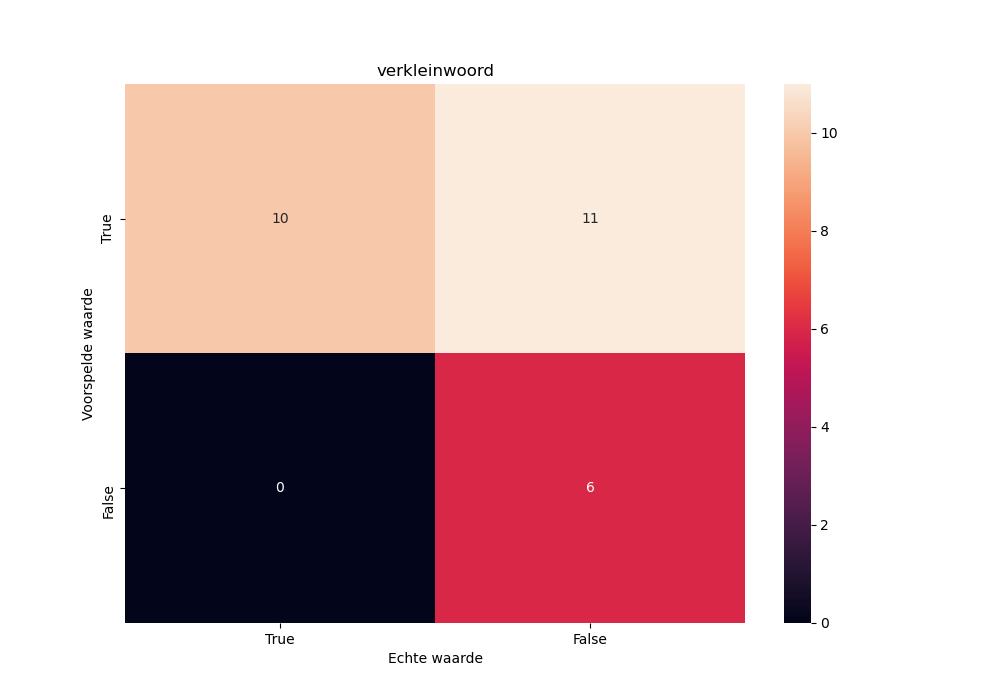
\includegraphics[width=1\textwidth]{./img/cfm_verkleinwoord}
	\caption{\label{fig:cfm_verkleinwoord} Resultaten \textit{confusion matrix} verkleinwoorden.}
\end{figure}


\subsection{Toonhoogte}
De testgevallen van de toonhoogte is te vinden in figuur~\ref{fig:cfm_pitch}. Daar is te zien dat er 5 correcte positieven zijn, 10 vals positieven, 7 valse negatieve en 32 correctie negatieven.
Hieruit kunnen we afleiden dat de applicatie een beetje werkt voor de toonhoogte, maar zich ook regelmatig vergist.

\begin{figure}
	\centering
	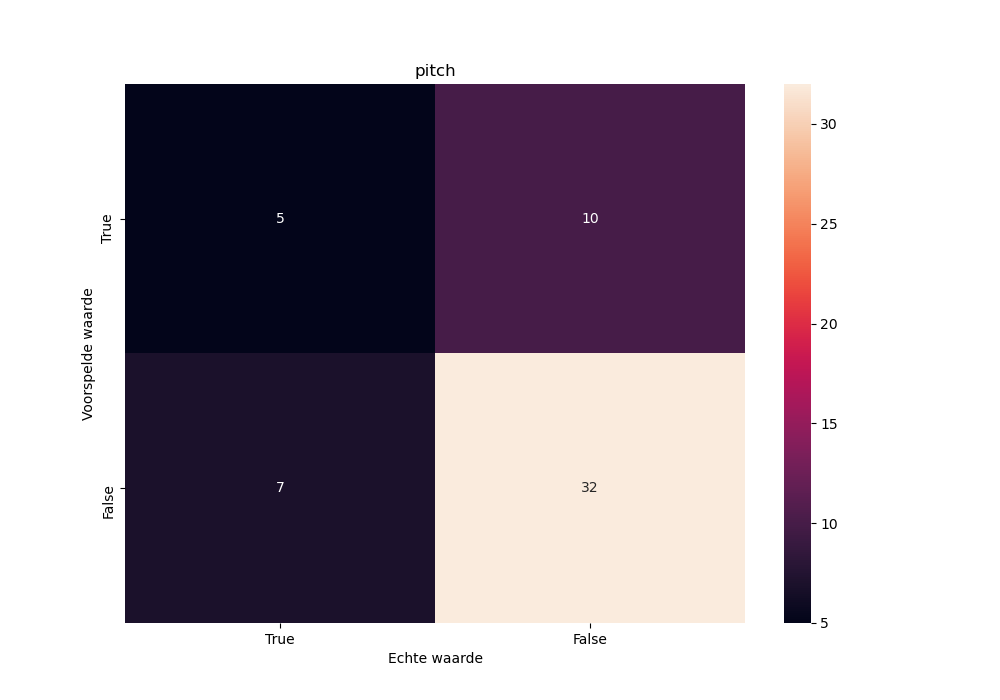
\includegraphics[width=1\textwidth]{./img/cfm_pitch}
	\caption{\label{fig:cfm_pitch} Resultaten \textit{confusion matrix} toonhoogte.}
\end{figure}

\subsection{Stemvolume}

De testgevallen van het stemvolume zijn te vinden in figuur~\ref{fig:cfm_pitch}. Daar is te zien dat er 4 correct-positieven zijn, 2 vals-positieven, 4 vals-negatieve en 44 correct-negatieven.
Hieruit kunnen we afleiden dat de applicatie goed werkt, maar toch een zekere foutmarge heeft.
\begin{figure}
	\centering
	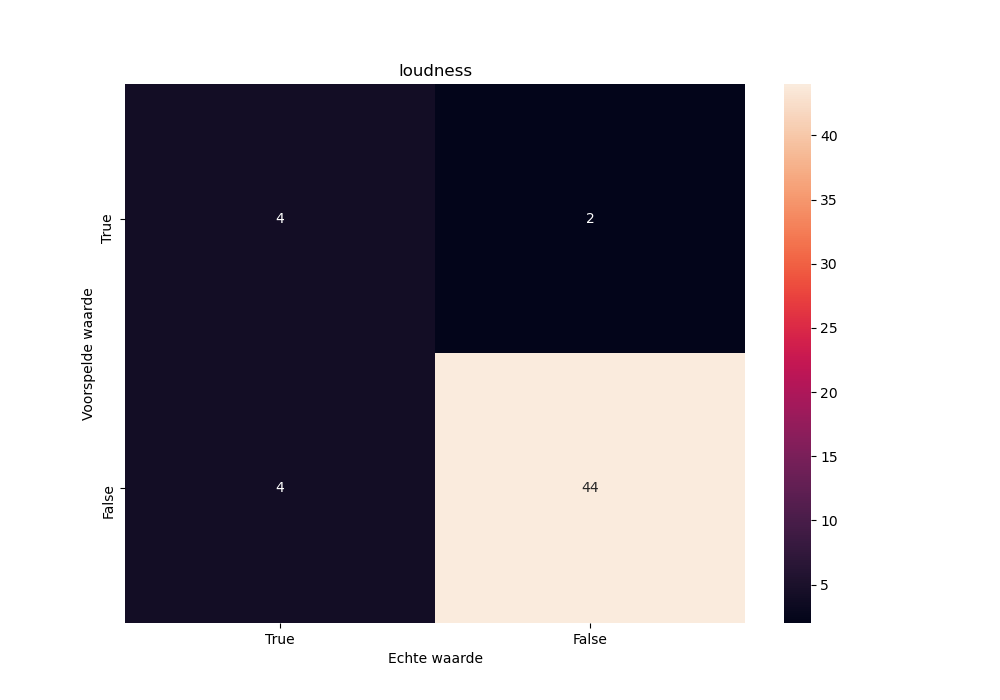
\includegraphics[width=1\textwidth]{./img/cfm_loudness}
	\caption{\label{fig:cfm_loudness} Resultaten \textit{confusion matrix} stemvolume.}
\end{figure}

\subsection{Algemeen besluit na testen}
A.d.h.v.\ deze \textit{confusion matrices} kan geconcludeerd worden dat er te weinig samples zijn om een beeld te vormen over de effectieve werking van de applicatie. Er moeten meer gevallen verzameld worden waarbij de toonhoogte of het stemvolume hoger is en waarbij er verkleinwoorden aanwezig zijn.

\section{Rollenspel}
Wanneer er een rollenspel gespeeld wordt, dan wordt de audio van beide personen geanalyseerd. Het is niet direct mogelijk om een stem weg te filteren als beide personen aanwezig zijn in de kamer. Alleen wanneer een van de twee personen significant verder staat van de microfoon, zal de applicatie die stem kunnen wegfilteren als achtergrondlawaai.

Toch kan er nog steeds geanalyseerd worden of er \textit{secondary baby talk} aanwezig is, dus de applicatie kan ook gebruikt worden om conversaties te oefenen.

\section{Is er aan de requirements voldaan?}
De \textit{requirements} zijn wel degelijk voldaan. Zo kan de applicatie de \textit{elderspeak} detecteren, weliswaar met een foutmarge die te lezen is hierboven.
Daarnaast kan de webapplicatie geïnstalleerd worden op een computer en heeft alles een een mooie lay-out gekregen.
Zo waren de applicatie en de scriptie ruimschoots op tijd klaar. Daarnaast is er ook een vervolghoofdstuk geschreven in Hoofdstuk~\ref{ch:vervolg} zodat dit onderzoek niet tevergeeft werd uitgevoerd.

\section{Live-demo}
Een live-demo van de applicatie kan gevonden worden via de volgende link op Vimeo: \url{https://vimeo.com/713225947/9ea9850566}.
In die video wordt gedemonstreerd hoe de applicatie werkt en er uit ziet.
